\documentclass[10pt]{beamer}

\usetheme{Madrid}
\usecolortheme{default}
\setbeamertemplate{navigation symbols}{}
\setbeamersize{text margin left=0.6cm,text margin right=0.6cm}

\usepackage{tikz}
\usetikzlibrary{automata,positioning,arrows.meta,calc,shapes.geometric}
\usepackage{amsmath,amssymb}
\usepackage{booktabs}
\usepackage{array}

\newcolumntype{L}[1]{>{\raggedright\arraybackslash}p{#1}}
\pdfstringdefDisableCommands{\def\translate#1{#1}}
\setbeamercovered{transparent=18}

\title{Pushdown Automata and Deterministic Parsing}
\subtitle{Memory with a Stack}
\author{Computer Science Theory}
\date{Slide Set 6}

\begin{document}

\begin{frame}
  \titlepage
\end{frame}

\begin{frame}{Learning Outcomes}
  \small
  By the end of this slide set, you should be able to:
  \begin{itemize}
    \item define a PDA and interpret transition labels and instantaneous descriptions;
    \item distinguish final-state and empty-stack acceptance;
    \item design and trace PDAs for matched counts, delimiters, and palindromes;
    \item explain both directions of the CFG--NPDA equivalence theorem;
    \item justify a PDA design using an invariant and test boundary cases;
    \item state the restrictions defining a deterministic PDA;
    \item distinguish regular, deterministic context-free, and context-free languages; and
    \item perform a simple shift--reduce parse and identify parser conflicts.
  \end{itemize}
\end{frame}

\begin{frame}{Road Map}
  \tableofcontents
\end{frame}

% ==========================================
% Part 1: NPDA foundations
% ==========================================
\section{Pushdown Automata: Definition and Design}

\begin{frame}{Why Add a Stack?}
  A finite automaton has only a constant amount of memory. It cannot retain the unbounded exact count
  needed for a language such as
  \[
    \{0^n1^n\mid n\ge0\}.
  \]
  \pause
  A stack provides unbounded but restricted memory:
  \begin{itemize}
    \item only the top symbol is directly accessible;
    \item symbols are removed in last-in, first-out order; and
    \item nesting and reversal naturally match stack behavior.
  \end{itemize}
  \pause
  \begin{block}{PDA intuition}
    A pushdown automaton is an NFA equipped with a stack. Its finite control chooses moves using the
    current state, the next input symbol (or $\varepsilon$), and the stack top.
  \end{block}
\end{frame}

\begin{frame}{PDA Architecture}
  \begin{center}
  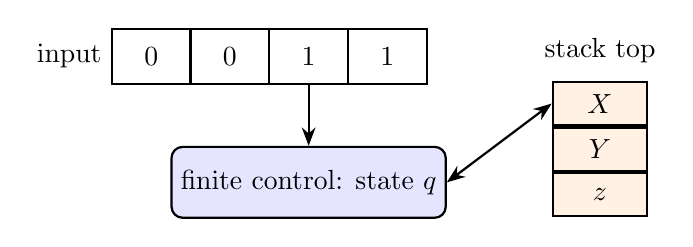
\begin{tikzpicture}[>=Stealth,thick]
    \foreach \x/\s in {0/0,1/0,2/1,3/1}{
      \draw (\x,1.7) rectangle +(1,0.7); \node at (\x+0.5,2.05) {\s};}
    \node[left] at (0,2.05) {input};
    \node[draw,rounded corners,fill=blue!10,minimum width=3.0cm,minimum height=0.9cm]
      (control) at (2.5,0.45) {finite control: state $q$};
    \draw[->] (2.5,1.7)--(control.north);
    \node[draw,fill=orange!10,minimum width=1.2cm,minimum height=0.55cm] (s1) at (6.2,1.45) {$X$};
    \node[draw,fill=orange!10,minimum width=1.2cm,minimum height=0.55cm,below=0cm of s1] (s2) {$Y$};
    \node[draw,fill=orange!10,minimum width=1.2cm,minimum height=0.55cm,below=0cm of s2] (s3) {$z$};
    \node[above=0.1cm of s1] {stack top};
    \draw[<->] (control.east)--(s1.west);
  \end{tikzpicture}
  \end{center}
  In one move, a PDA may consume one input symbol or consume nothing, pop the top stack symbol,
  replace it by a finite string, and change state.
  \pause
  The input head moves only to the right when a symbol is consumed.
  The stack is not random-access memory: even reading below the top requires
  first removing what lies above it.
\end{frame}

\begin{frame}{Formal Definition and Textbook Conventions}
  \small
  We use the Linz-style 7-tuple
  \[
    M=(Q,\Sigma,\Gamma,\delta,q_0,z,F),
  \]
  \pause
  where
  \begin{itemize}
    \item $Q$ is a finite nonempty state set; $\Sigma$ and $\Gamma$ are finite
      input and stack alphabets, respectively;
    \item $q_0\in Q$ is the start state, $z\in\Gamma$ is the initial stack symbol, and $F\subseteq Q$;
    \item
      \[
        \delta:Q\times(\Sigma\cup\{\varepsilon\})\times\Gamma
        \to\mathcal{P}_{\mathrm{fin}}(Q\times\Gamma^*).
      \]
  \end{itemize}
  Here $\mathcal{P}_{\mathrm{fin}}$ means finite subsets, so the machine has
  finitely many transition alternatives. $\varepsilon$ is not an alphabet symbol.
  Sipser commonly uses a six-component convention with an initially empty stack and permits a move
  not to inspect a stack symbol. These conventions are computationally equivalent.
  \pause
  \begin{alertblock}{Convention used below}
    The stack top is written on the left, and every displayed transition pops one stack symbol before
    pushing its replacement.
  \end{alertblock}
  An empty stack enables no further moves in this convention.
\end{frame}

\begin{frame}{Reading PDA Transition Labels}
  We abbreviate a move by
  \[
    a,X\to\gamma.
  \]
  \pause
  It means: read $a$ (or read nothing if $a=\varepsilon$), pop $X$, and push
  $\gamma$. With the top on the left, the first symbol of $\gamma$ becomes the new top.
  \begin{center}
  \begin{tabular}{L{3.2cm}L{7.0cm}}
    \toprule
    Label & Effect \\
    \midrule
    $0,z\to0z$ & read $0$ and place a marker above the bottom symbol \\
    $0,0\to00$ & read $0$ and add one more marker \\
    $1,0\to\varepsilon$ & read $1$ and remove one marker \\
    $\varepsilon,z\to z$ & change state without consuming input or changing the stack \\
    \bottomrule
  \end{tabular}
  \end{center}
  An NPDA may have several enabled moves and accepts if at least one computation branch accepts.
  Unlisted transitions mean $\varnothing$ (no move), not an implicit self-loop.
\end{frame}

\begin{frame}{Instantaneous Descriptions}
  An instantaneous description (ID) is a triple
  \[
    (q,w,u),
  \]
  \pause
  where $q$ is the current state, $w$ is the unread input, and $u$ is the stack content with top on the left.
  If $(p,\gamma)\in\delta(q,a,X)$, then
  \[
    (q,aw,X\alpha)\vdash(p,w,\gamma\alpha),
  \]
  where $a\in\Sigma\cup\{\varepsilon\}$ and $aw=w$ when $a=\varepsilon$.
  \pause
  \begin{block}{Reflexive transitive closure}
    $(q,w,u)\vdash^*(p,x,v)$ means that zero or more PDA moves transform the first ID into the second.
  \end{block}
\end{frame}

\begin{frame}{Two Acceptance Conventions}
  A computation starts in $(q_0,w,z)$ and must consume the entire input.
  \begin{block}{Acceptance by final state}
    \[
      (q_0,w,z)\vdash^*(q_f,\varepsilon,u)
      \quad\text{for some }q_f\in F,\ u\in\Gamma^*.
    \]
  \end{block}
  \pause
  \begin{block}{Acceptance by empty stack}
    \[
      (q_0,w,z)\vdash^*(q,\varepsilon,\varepsilon)
      \quad\text{for some }q\in Q.
    \]
  \end{block}
  For NPDAs, both conventions define exactly the context-free languages.
  This means equivalent machines can be constructed, not that the two
  tests give the same language for an unchanged machine.
\end{frame}

\begin{frame}{Acceptance, Blocking, and Infinite Branches}
  \small
  Acceptance means that a \emph{finite} successful computation exists.
  A blocked branch is unsuccessful unless its current ID already satisfies
  the chosen acceptance condition.
  \begin{block}{Three different situations}
    \begin{itemize}
      \item $(q_f,\varepsilon,Xz)$ accepts by final state, but not by empty stack.
      \item $(q,\varepsilon,z)$ is not an empty stack: $z$ is a real symbol.
      \item $(q_f,a,\varepsilon)$ does not accept: input $a$ remains, and
        our convention enables no move without a stack top.
    \end{itemize}
  \end{block}
  \pause
  An $\varepsilon$-cycle such as $\delta(q,\varepsilon,z)=\{(q,z)\}$ can
  produce an infinite branch. It does not consume input or itself establish acceptance.
  \begin{alertblock}{Do not confuse recognition with a terminating simulation}
    One infinite branch does not invalidate another accepting branch.
    Conversely, repeatedly exploring one branch may never settle membership.
    CFL membership is decidable using a CFG and a terminating parser such as CYK.
  \end{alertblock}
\end{frame}


\begin{frame}{A PDA Design Checklist}
  \small
  \begin{enumerate}
    \item Specify the alphabet, acceptance mode, and any explicit endmarker.
    \item Decide what each stack symbol records: a count, delimiter, or
      symbol awaiting a reversed match.
    \item Use states for phases; the stack alone need not enforce input order.
    \item Write an invariant relating the consumed prefix, state, and stack.
    \item List moves for \emph{every relevant stack top}, including the
      bottom marker. Leave invalid cases without a move.
    \item Test $\varepsilon$, the shortest valid word, a mismatch, and a
      valid word with an invalid extension; then prove both inclusions.
  \end{enumerate}
  \pause
  \begin{block}{What nondeterminism adds}
    A branch can guess a phase boundary or grammar production and then
    verify it. The guess cannot inspect the future, and an incorrect branch
    must never accept. Deterministic designs need an observable basis for
    each choice, such as a delimiter or the first symbol of a new block.
  \end{block}
\end{frame}

\begin{frame}{Worked PDA: $\{0^n1^n\mid n\ge0\}$}
  \begin{center}
  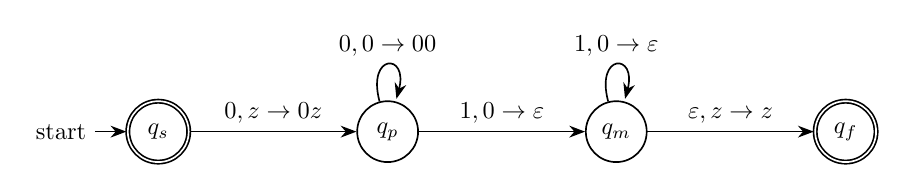
\begin{tikzpicture}[->,>=Stealth,auto,node distance=2.4cm,semithick,
      scale=0.88,transform shape]
    \node[state,initial,accepting] (qs) {$q_s$};
    \node[state,right=of qs] (qp) {$q_p$};
    \node[state,right=of qp] (qm) {$q_m$};
    \node[state,accepting,right=of qm] (qf) {$q_f$};
    \path (qs) edge node {$0,z\to0z$} (qp)
          (qp) edge[loop above] node {$0,0\to00$} (qp)
          (qp) edge node {$1,0\to\varepsilon$} (qm)
          (qm) edge[loop above] node {$1,0\to\varepsilon$} (qm)
          (qm) edge node {$\varepsilon,z\to z$} (qf);
  \end{tikzpicture}
  \end{center}
  \pause
  \begin{exampleblock}{Trace on $0011$}
    \[
    \begin{aligned}
      (q_s,0011,z)&\vdash(q_p,011,0z)
      \vdash(q_p,11,00z)\\
      &\vdash(q_m,1,0z)
      \vdash(q_m,\varepsilon,z)
      \vdash(q_f,\varepsilon,z).
    \end{aligned}
    \]
  \end{exampleblock}
  The states enforce the input order $0^*1^*$; the stack enforces equal counts.
  State $q_s$ accepts $\varepsilon$; $q_f$ has no outgoing moves.
\end{frame}

\begin{frame}{Why the Matched-Count PDA Is Correct}
  \small
  The control state records the phase; the stack records the difference
  between the counts read so far.
  \begin{block}{Invariant along every nonblocked run}
    In $q_p$, the consumed prefix is $0^k$ and the stack is $0^kz$,
    where $k\ge1$. In $q_m$, the prefix is $0^k1^j$ and the stack is
    $0^{k-j}z$, where $1\le j\le k$.
    Each displayed transition preserves these statements.
  \end{block}
  \pause
  \textbf{Soundness.} The initial final state accepts only $\varepsilon$.
  To reach $q_f$, $q_m$ must expose $z$, so $j=k$. Acceptance additionally
  requires exhausted input. Thus only $0^k1^k$ can be accepted.
  \pause
  \par\smallskip
  \textbf{Completeness.} For any $k\ge1$, push exactly $k$ markers on the
  zeros, pop them on the $k$ ones, then enter $q_f$. The case $k=0$ accepts
  in $q_s$ without a move.
  \begin{exampleblock}{Boundary checks}
    $001$ leaves a marker; $00111$ leaves input even after reaching $q_f$;
    $0101$ cannot return to the push phase. All three are rejected.
  \end{exampleblock}
\end{frame}

\begin{frame}{NPDA for Even-Length Palindromes}
  The language
  \[
    \{ww^R\mid w\in\{a,b\}^*\}
  \]
  \pause
  is recognized by guessing the midpoint and then checking the guess.
  \begin{center}
  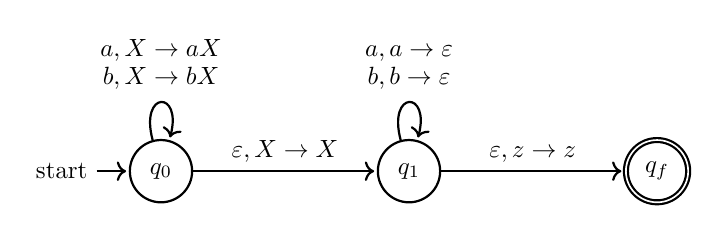
\begin{tikzpicture}[shorten >=1pt,node distance=3.5cm,on grid,auto,thick,scale=0.9,transform shape]
    \node[state,initial] (q0) {$q_0$};
    \node[state,right=of q0] (q1) {$q_1$};
    \node[state,accepting,right=of q1] (qf) {$q_f$};
    \path[->]
      (q0) edge[loop above] node {$\begin{matrix}a,X\to aX\\[-1pt]b,X\to bX\end{matrix}$} (q0)
           edge node {$\varepsilon,X\to X$} (q1)
      (q1) edge[loop above] node {$\begin{matrix}a,a\to\varepsilon\\[-1pt]b,b\to\varepsilon\end{matrix}$} (q1)
           edge node {$\varepsilon,z\to z$} (qf);
  \end{tikzpicture}
  \end{center}
  Here $X$ ranges over $\Gamma=\{a,b,z\}$; $z\notin\{a,b\}$.
  For each word in the language, a branch guesses the midpoint and accepts.
  A nonmember has no accepting branch.
\end{frame}

\begin{frame}{Tracing the Palindrome NPDA on $abba$}
  One accepting branch is
  \[
  \begin{aligned}
    (q_0,abba,z)
      &\vdash(q_0,bba,az) &&\text{push }a\\
      &\vdash(q_0,ba,baz) &&\text{push }b\\
      &\vdash(q_1,ba,baz) &&\text{guess the midpoint}\\
      &\vdash(q_1,a,az) &&\text{match and pop }b\\
      &\vdash(q_1,\varepsilon,z) &&\text{match and pop }a\\
      &\vdash(q_f,\varepsilon,z). &&
  \end{aligned}
  \]
  \pause
  Guesses made too early or too late eventually block or leave unmatched input/stack symbols.
  To accept both parities, add midpoint moves consuming one symbol without
  changing the stack. For odd lengths only, replace the empty midpoint moves.
\end{frame}

\begin{frame}{A Deterministic Stack Pattern: Balanced Parentheses}
  \small
  Here we explicitly supply $w\dashv$, where $\dashv\notin\{(,)\}$ is a
  fresh right endmarker. It is a real input symbol, unlike $\varepsilon$.
  A PDA can recognize balanced parentheses deterministically:
  \begin{enumerate}
    \item on input $($, push a marker;
    \item on input $)$, pop one marker; reject if no marker is available;
    \item at the endmarker, accept exactly when only the bottom marker remains.
  \end{enumerate}
  \pause
  \begin{exampleblock}{Trace on $(()())$, with $X$ for an unmatched opener}
    \[
      z\to Xz\to XXz\to Xz\to XXz\to Xz\to z.
    \]
  \end{exampleblock}
  In a work state $q$, use $(,A\to XA$ for $A\in\{X,z\}$,
  $),X\to\varepsilon$, and $\dashv,z\to z$ to a final state.
  No other moves are enabled. The bottom marker cannot match a closer.
  This is the machine analogue of the CFG $S\to(S)S\mid\varepsilon$.
\end{frame}

% ==========================================
% Part 2: Equivalence
% ==========================================
\section{Equivalence of CFGs and NPDAs}

\begin{frame}{The Equivalence Theorem}
  \begin{block}{Theorem}
    A language is context-free iff some nondeterministic pushdown automaton recognizes it.
  \end{block}
  The proof has two constructive directions:
  \[
    \mathrm{CFG}\Longrightarrow\mathrm{NPDA}
    \qquad\text{and}\qquad
    \mathrm{NPDA}\Longrightarrow\mathrm{CFG}.
  \]
  \pause
  \begin{itemize}
    \item A CFG derivation can be simulated as nondeterministic stack expansion.
    \item A PDA's stack-balanced computations can be named by grammar variables.
  \end{itemize}
  Thus grammars and NPDAs are two views of the same language class: generation versus recognition.
\end{frame}

\begin{frame}{CFG $\Rightarrow$ NPDA: Construction}
  \small
  Given a CFG $G=(V,T,S,P)$, build an NPDA that accepts by empty stack:
  \begin{enumerate}
    \item initialize the stack with $S$ above a bottom marker;
    \item if the top is a variable $A$, nondeterministically choose $A\to\beta$ and replace $A$ by $\beta$;
    \item if the top is terminal $a$ and the next input symbol is $a$, read it and pop it;
    \item whenever only the bottom marker remains, allow it to be popped.
      Empty-stack acceptance additionally requires exhausted input.
  \end{enumerate}
  \pause
  \begin{block}{Invariant}
    If $u$ is the consumed prefix and $\alpha$ is the stack above the bottom
    marker, then $S\Rightarrow^*u\alpha$ by leftmost expansion.
    It is $u\alpha$, not necessarily $\alpha$ alone, that is a sentential form.
  \end{block}
  A bad choice may leave $\alpha$ unable to derive the unread suffix.
  Only one successful branch is needed. With top on the left, replacing
  $A$ by $\beta$ puts its leftmost symbol on top.
\end{frame}

\begin{frame}{Tracing the CFG Simulation}
  For $S\to0S1\mid\varepsilon$ on input $0011$, show the unread input before the stack:
  \[
  \begin{array}{ccl}
    0011 &;& Sz\\
    0011 &;& 0S1z\\
    011  &;& S1z\\
    011  &;& 0S11z\\
    11   &;& S11z\\
    11   &;& 11z\\
    1    &;& 1z\\
    \varepsilon &;& z\\
    \varepsilon &;& \varepsilon.
  \end{array}
  \]
  \pause
  Variable expansions are $\varepsilon$-moves; terminal matches consume input; the final move pops $z$.
  The accepting branch mirrors the derivation
  $S\Rightarrow0S1\Rightarrow00S11\Rightarrow0011$.
\end{frame}



\begin{frame}{NPDA $\Rightarrow$ CFG: The Core Idea}
  \small
  First convert the NPDA to empty-stack acceptance. The difficulty is that
  its stack can grow without bound; we cannot make one variable per full stack.
  \begin{block}{Name a stack-removal task instead}
    The variable $[pAq]$ describes input consumed while starting in state $p$
    with top $A$, removing $A$ and everything pushed above it, and first
    exposing the lower stack in state $q$. The lower stack is untouched.
  \end{block}
  \pause
  If a move replaces $A$ by $BC$, then all of $B$'s work must finish before
  $C$'s work begins. A grammar production joins those two tasks, guessing
  the intermediate state. There are only finitely many state/symbol triples.
  \pause
  \[
    S\to[q_0zq]\quad\text{for every }q\in Q.
  \]
  These alternatives describe exactly the computations that remove the
  initial stack. Induction relates derivation trees to nested stack removals.
  The appendix supplies the precise productions and a worked conversion.
\end{frame}

% ==========================================
% Part 3: Determinism
% ==========================================
\section{Deterministic PDAs and DCFLs}

\begin{frame}{What Makes a PDA Deterministic?}
  \small
  A PDA is deterministic when, for every state $q$ and stack top $X$:
  \begin{enumerate}
    \item for each $a\in\Sigma\cup\{\varepsilon\}$, at most one move is available; and
    \item if an $\varepsilon$-move is available, no input-consuming move is available for any next symbol.
  \end{enumerate}
  \pause
  Formally,
  \[
    |\delta(q,a,X)|\le1,
  \]
  and $\delta(q,\varepsilon,X)\ne\varnothing$ implies
  $\delta(q,a,X)=\varnothing$ for every $a\in\Sigma$.
  \pause
  \begin{block}{Consequence}
    For a fixed input, a DPDA has at most one computation path. An NPDA may explore many incompatible
    stack strategies and accepts if one succeeds.
  \end{block}
  A \textbf{DCFL} is a language accepted by a DPDA by final state.
  This definition does not require an endmarker; marked inputs will be
  identified explicitly. Determinism does not guarantee halting.
\end{frame}

\begin{frame}{Known Midpoint Versus Guessed Midpoint}
  Compare two languages:
  \[
    L_1=\{wcw^R\mid w\in\{a,b\}^*\},
    \qquad
    L_2=\{ww^R\mid w\in\{a,b\}^*\}.
  \]
  \pause
  \begin{itemize}
    \item $L_1$ is a DCFL: push before the marker $c$, then deterministically pop and compare after $c$.
    \item $L_2$ is context-free but not deterministic context-free; an NPDA guesses where the second half begins.
  \end{itemize}
  \pause
  \begin{alertblock}{Proof caution}
    Failure of the obvious DPDA design is not itself a proof that $L_2$ is not a DCFL. The non-DCFL
    claim is a theorem established using deeper closure or structural arguments.
  \end{alertblock}
\end{frame}

\begin{frame}{Worked DPDA: A Marked Midpoint}
  \small
  For $L=\{wcw^R:w\in\{a,b\}^*\}$ use states $p$ (push), $m$ (match),
  and final state $f$. Initially the state is $p$ and the stack is $z$.
  With $x\in\{a,b\}$ and $X\in\{a,b,z\}$, the complete move list is
  \[
    \begin{aligned}
      \delta(p,x,X)&=\{(p,xX)\},&
      \delta(p,c,X)&=\{(m,X)\},\\
      \delta(m,x,x)&=\{(m,\varepsilon)\},&
      \delta(m,\varepsilon,z)&=\{(f,z)\}.
    \end{aligned}
  \]
  All other entries are empty; $f$ has no outgoing moves. No endmarker is used.
  \pause
  \begin{block}{Why it works, and why it is deterministic}
    After reading $w$ before $c$, the stack is $w^Rz$.
    After $c$, each input symbol must match the top, so acceptance requires
    exactly $w^R$. The only empty move is at $(m,z)$, where no consuming
    move is enabled. There is never a choice between pushing and matching.
  \end{block}
  \pause
  \textbf{Tests:} $c$ and $abcba$ accept; $\varepsilon$, $abca$, and $cc$
  reject. On $cc$ the run may reach $f$ with unread $c$, which is not acceptance.
\end{frame}

\begin{frame}{Language-Class Hierarchy}
  \small
  \begin{columns}[T]
    \column{0.38\textwidth}
    \centering
    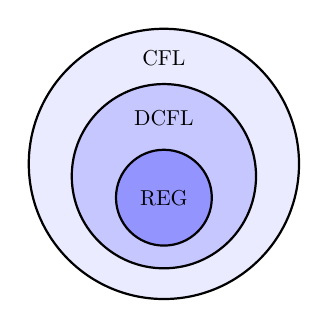
\begin{tikzpicture}[scale=0.78,transform shape]
      \draw[thick,fill=blue!8] (0,0) circle (2.2cm);
      \node at (0,1.72) {CFL};
      \draw[thick,fill=blue!22] (0,-0.2) circle (1.5cm);
      \node at (0,0.75) {DCFL};
      \draw[thick,fill=blue!42] (0,-0.55) circle (0.78cm);
      \node at (0,-0.55) {REG};
    \end{tikzpicture}

    \column{0.60\textwidth}
    \[
      \mathrm{REG}\subsetneq\mathrm{DCFL}\subsetneq\mathrm{CFL}.
    \]
    \begin{itemize}
      \item $\{0^n1^n:n\ge0\}$ is a nonregular DCFL.
      \item $\{ww^R:w\in\{a,b\}^*\}$ is a CFL but not a DCFL.
      \item Every DCFL has an unambiguous CFG.
      \item The converse fails: $S\to aSa\mid bSb\mid\varepsilon$ is
        unambiguous, but its language is not a DCFL.
    \end{itemize}
  \end{columns}
  \pause
  To simulate any DFA, keep $z$ unchanged on every move and copy the DFA's
  states, transitions, and final states. Thus every regular language is a DCFL.
\end{frame}


\begin{frame}{Acceptance Conventions Under Determinism}
  \small
  Final-state and empty-stack acceptance are equivalent for NPDAs but not interchangeable for DPDAs.
  \begin{block}{Why empty-stack DPDAs are restricted}
    If a DPDA accepts $x$ by empty stack, it has no stack content with which to continue processing a
    proper extension $xy$. Deterministic empty-stack languages are therefore prefix-free.
  \end{block}
  \textbf{Counterexample:} $\{a,aa\}$ is regular and hence a DCFL, but not
  prefix-free, so no unmarked empty-stack DPDA accepts it.
  \pause
  With a fresh endmarker, we instead supply $w\dashv$ and recognize
  $L\dashv=\{w\dashv:w\in L\}$. A suitably arranged final-state DPDA can
  consume $\dashv$ at its acceptance decision and then drain the stack.
  The marker distinguishes end of input from a prefix that might continue.
  \par\smallskip
  Do not silently transfer a claim about $L\dashv$ to empty-stack acceptance of $L$.
\end{frame}

% ==========================================
% Part 4: Parsing
% ==========================================
\section{Deterministic Parsing}

\begin{frame}{Why Parsing Looks Like a DPDA}
  A parser reads tokens left to right while its stack records unfinished syntactic structure.
  \begin{itemize}
    \item The finite control represents a parser state or set of viable grammar situations.
    \item The stack stores grammar symbols or states for nested constructs.
    \item A fixed-size lookahead buffer can be stored in finite control;
      together with the parser state, it determines the next action.
  \end{itemize}
  \pause
  \begin{block}{Endmarker}
    A fresh symbol such as $\dashv$ or \texttt{\$} marks the actual end of the token stream and allows
    acceptance to be decided deterministically.
  \end{block}
\end{frame}

\begin{frame}{Top-Down and Bottom-Up Parsing}
  \begin{center}
  \begin{tabular}{L{5.0cm}L{5.0cm}}
    \toprule
    Top-down / LL-style & Bottom-up / LR-style \\
    \midrule
    Starts from $S$ and predicts productions. & Starts from the input and recognizes handles. \\
    Constructs a leftmost derivation. & Constructs a rightmost derivation in reverse. \\
    Must choose a production before seeing its full body. & Delays a decision until a right-hand side is recognized. \\
    Simple and natural for hand-written parsers. & Handles a broader range of programming-language grammars. \\
    \bottomrule
  \end{tabular}
  \end{center}
  Both approaches require grammar restrictions or parser tables that make each decision unique.
\end{frame}


\begin{frame}{Handles and Rightmost Derivations}
  \small
  In a right-sentential form, a \textbf{handle} is an occurrence of a production right-hand side whose
  reduction reverses one step of a rightmost derivation.
  For
  \[
    S\to aSb\mid ab,
  \]
  \pause
  a rightmost derivation of $aabb$ is
  \[
    S\Rightarrow aSb\Rightarrow aabb.
  \]
  Reversing it gives reductions (write $\rightsquigarrow$ to distinguish
  them from grammar derivation steps):
  \[
    aabb\rightsquigarrow aSb\rightsquigarrow S.
  \]
  First the middle $ab$ is the handle; after that reduction, the entire $aSb$ is the handle.
\end{frame}

\begin{frame}{Shift--Reduce Parser Actions}
  A bottom-up parser repeatedly chooses one action:
  \begin{description}
    \item[Shift:] move the next token onto the stack;
    \item[Reduce:] replace a handle $\beta$ by $A$ when $A\to\beta$ is a
      production, without consuming input;
    \item[Accept:] the stack represents $S$ and the lookahead is the endmarker;
    \item[Error:] no valid continuation exists.
  \end{description}
  An LR($k$) parser scans left to right and uses at most $k$ lookahead symbols to construct a rightmost
  derivation in reverse.
\end{frame}

\begin{frame}{Worked Shift--Reduce Trace for $aabb$}
  Grammar: $S\to aSb\mid ab$.
  \begin{center}
  \begin{tabular}{ccl}
    \toprule
    Stack & Unread input & Action \\
    \midrule
    $\varepsilon$ & $aabb\dashv$ & shift $a$ \\
    $a$ & $abb\dashv$ & shift $a$ \\
    $aa$ & $bb\dashv$ & shift $b$ \\
    $aab$ & $b\dashv$ & reduce $ab\to S$ \\
    $aS$ & $b\dashv$ & shift $b$ \\
    $aSb$ & $\dashv$ & reduce $aSb\to S$ \\
    $S$ & $\dashv$ & accept \\
    \bottomrule
  \end{tabular}
  \end{center}
  Parser states—not only visible grammar symbols—normally determine when a reduction is valid.
\end{frame}

\begin{frame}{Parser Conflicts}
  \small
  \begin{alertblock}{Shift--reduce conflict}
    The parser cannot choose uniquely between shifting the next token and reducing the current stack suffix.
  \end{alertblock}
  \pause
  \begin{alertblock}{Reduce--reduce conflict}
    Two different productions appear eligible for reduction.
  \end{alertblock}
  Conflicts may indicate:
  \begin{itemize}
    \item an ambiguous grammar;
    \item insufficient lookahead for the chosen parsing method; or
    \item a grammar that needs restructuring or explicit precedence/associativity declarations.
  \end{itemize}
  An ambiguous grammar is not LR($k$) for any fixed $k$. Precedence rules
  can select one interpretation, but this adds a disambiguation policy;
  it does not make the original grammar unambiguous.
\end{frame}


% ==========================================
% Review
% ==========================================
\section{Review and Exercises}

\begin{frame}{Checkpoint Exercises I: PDA Mechanics}
  \small
  \begin{enumerate}
    \item Trace the $\{0^n1^n\}$ PDA on $000111$. Where does it block on $00111$?
    \item Give an accepting ID sequence for the palindrome NPDA on $baab$.
    \item Modify the palindrome NPDA to accept odd-length palindromes as well,
      and explain the change needed for odd lengths only.
    \item Design a DPDA for $\{wcw^R\mid w\in\{a,b\}^*\}$.
    \item Explain why final-state acceptance requires the input to be exhausted.
    \item Convert, at proof-sketch level, an empty-stack NPDA to final-state acceptance.
  \end{enumerate}
\end{frame}

\begin{frame}{Checkpoint Exercises II: Theory and Parsing}
  \small
  \begin{enumerate}
    \item Place each language in the smallest class: regular, DCFL, CFL, or non-CFL.
      Use $n\ge0$ and $w\in\{a,b\}^*$:
      \[
        0^*1^*,\quad \{0^n1^n\},\quad \{ww^R\},\quad \{a^n b^n c^n\}.
      \]
    \item Why does an unambiguous CFG not necessarily define a DCFL?
    \item Use the state-pair meaning to explain $[pAq]$ in one sentence.
    \item Identify the two handles in $aabb\rightsquigarrow aSb\rightsquigarrow S$.
    \item What is the difference between a shift--reduce conflict and a reduce--reduce conflict?
    \item Why is an endmarker especially useful for deterministic acceptance?
  \end{enumerate}
\end{frame}

\begin{frame}{Common Mistakes to Avoid}
  \begin{itemize}
    \item Forgetting which end of the written stack is the top.
    \item Treating an $\varepsilon$-move as if it consumed an input symbol.
    \item Accepting merely because a final state is reached while input remains.
    \item Assuming all nondeterministic branches must accept; one accepting branch is sufficient.
    \item Assuming final-state and empty-stack acceptance remain equivalent for DPDAs.
    \item Claiming a language is non-DCFL only because one deterministic design attempt failed.
    \item Reducing the wrong substring during a shift--reduce trace instead of the actual handle.
  \end{itemize}
\end{frame}

\begin{frame}{Summary}
  \begin{itemize}
    \item A PDA combines finite control with an unbounded LIFO stack.
    \item NPDAs accept by the existence of a successful computation branch.
    \item Final-state and empty-stack acceptance are equivalent for NPDAs.
    \item CFGs and NPDAs define exactly the context-free languages.
    \item Determinism is strictly weaker for PDAs: $\mathrm{REG}\subsetneq\mathrm{DCFL}\subsetneq\mathrm{CFL}$.
    \item Endmarkers and deterministic stacks connect DPDAs to practical LL/LR parsing.
    \item Shift--reduce parsing reconstructs a rightmost derivation in reverse.
  \end{itemize}
\end{frame}

\appendix
\section{Appendix: Challenges, Proofs, and Further Results}

\begin{frame}{Appendix Guide}
  \small
  The main sequence develops PDA mechanics, both equivalence directions,
  determinism, and the ideas behind predictive and shift--reduce parsing.
  The following material is optional enrichment, organized for self-study:
  \begin{itemize}
    \item checkpoint answers, followed by five solved construction challenges;
    \item acceptance conversions and exact CFG--NPDA proof details;
    \item DCFL closure and the complement-construction pitfall;
    \item bounded stacks, two-stack machines, and visibly pushdown automata;
    \item a predictive parse, concrete conflicts, and a complete LR table.
  \end{itemize}
  \begin{block}{Suggested use}
    Attempt each challenge before revealing its solution. The main lecture
    retains both equivalence directions at proof-sketch level; the detailed
    conversions and parser machinery can be assigned as follow-up reading.
    Exercise sources and editions are identified explicitly below.
  \end{block}
\end{frame}

\subsection{Checkpoint Solutions}

\begin{frame}{Hints and Short Answers I}
  \small
  \begin{itemize}
    \item On $00111$, the stack reaches $z$ while one $1$ remains, so no accepting complete-input ID exists.
    \item For $baab$, push $b,a$, guess the midpoint, then pop on $a,b$.
    \item Add transitions consuming one $a$ or $b$ without changing the stack.
      Retain the empty midpoint moves for both parities; remove them for odd lengths only.
    \item For $wcw^R$, push before $c$, change phase on $c$, and then pop matching symbols.
    \item A final state reached with unread input is not an accepting ID under the language definition.
    \item Protect the simulated stack with a fresh bottom marker and enter a new final state when that marker is exposed.
  \end{itemize}
\end{frame}

\begin{frame}{Hints and Short Answers II}
  \small
  \begin{itemize}
    \item The four classes are respectively regular; DCFL but nonregular; CFL but not DCFL; and non-CFL.
    \item Unambiguity is necessary for deterministic context-freeness but not sufficient; palindromes provide a standard example.
    \item $[pAq]$ generates strings that remove $A$ while taking the PDA from state $p$ to state $q$ without disturbing the lower stack.
    \item The handles are the middle $ab$, followed by the entire $aSb$.
    \item Shift--reduce offers one shift and one reduction; reduce--reduce offers two reductions.
    \item The endmarker distinguishes a completed input from a prefix that might receive more symbols.
  \end{itemize}
\end{frame}

\subsection{Solved Construction Challenges}

\begin{frame}{Challenge Sources and How to Use the Solutions}
  \small
  The prompts below are paraphrased; the worked solutions and explanations
  are written for this course, not reproduced from a solutions manual.
  \begin{center}
  \begin{tabular}{L{4.9cm}L{5.5cm}}
    \toprule
    Challenge & Source / status \\
    \midrule
    1. Choose a count comparison & Sipser, 2nd ed., Exercise 2.10
      (language from 2.9) \\
    2. Cancel opposite symbols & Sipser, 2nd ed., Exercise 2.7(a),
      referring to 2.6(a) \\
    3. Find a reversed substring & Sipser, 2nd ed., Exercise 2.7(c),
      referring to 2.6(c) \\
    4. Combine a PDA and a DFA & Sipser, 2nd ed., Problem 2.18(a) \\
    5. Split a count across blocks & Additional course practice;
      no textbook exercise number claimed \\
    \bottomrule
  \end{tabular}
  \end{center}
  \cite{sipser-second} supplies these edition-specific references.
  Linz's PDA/ID viewpoint guides the phase descriptions and invariants.
  \begin{block}{Before reading an answer}
    Choose the acceptance convention, state the stack invariant, and test
    the empty and zero-count cases. Then justify both inclusions.
  \end{block}
\end{frame}

\begin{frame}{Challenge 1: Guess Which Equality to Check}
  \small
  \textbf{Task:} build an NPDA for
  \[
    L=\{a^i b^j c^k:i=j\text{ or }j=k,\quad i,j,k\ge0\}.
  \]
  \pause
  \begin{block}{Solution: make one initial nondeterministic choice}
    Both branches enforce the order $a^*b^*c^*$ and consume all input.
    \begin{itemize}
      \item \textbf{Check $i=j$:} push a marker per $a$, pop one per $b$,
        and permit the $c$-phase only after all markers are removed.
        Once in that phase, read any number of $c$'s.
      \item \textbf{Check $j=k$:} read the initial $a$'s without changing
        the stack, push on $b$, and pop on $c$.
    \end{itemize}
    Use a protected bottom marker. A branch accepts only in an appropriate
    final state with no unmatched markers; phases may have length zero.
  \end{block}
  \pause
  \textbf{Why it works:} a successful branch certifies one equality.
  Conversely, if either equality holds, its branch can finish successfully.
  \par\smallskip
  \textbf{Checks:} $aabbc$ uses the first branch; $abbcc$ uses the second;
  $abbc$ fails both; $\varepsilon$ succeeds in both.
  Several accepting branches are permitted---acceptance means logical OR.
\end{frame}

\begin{frame}{Challenge 2: More $a$'s Than $b$'s, in Any Order}
  \small
  \textbf{Task:} recognize $L=\{w\in\{a,b\}^*:|w|_a>|w|_b\}$.
  A push-then-pop design is insufficient: the symbols may interleave.
  \pause
  \textbf{Solution:} in a work state $q$, use the following replacements.
  An entry $\gamma$ means $\delta(q,\text{input},X)=\{(q,\gamma)\}$.
  \[
    \begin{array}{c|ccc}
      \text{input}\backslash\text{top }X & z&A&B\\\hline
      a&Az&AA&\varepsilon\\
      b&Bz&\varepsilon&BB
    \end{array}
  \]
  Supply a fresh endmarker $\dashv$. The only move on it is
  $\delta(q,\dashv,A)=\{(f,A)\}$, where $f$ is final and has no outgoing moves.
  This DPDA accepts exactly $L\dashv$.
  \pause
  \begin{block}{Invariant: cancel opposite symbols}
    For the consumed prefix $u$, let $d=|u|_a-|u|_b$.
    The stack is $A^dz$ if $d>0$, $B^{-d}z$ if $d<0$, and $z$ if $d=0$.
    Each table entry updates this signed difference by $+1$ or $-1$.
  \end{block}
  At the end, top $A$ is equivalent to $d>0$. Thus $ababa$ succeeds,
  while $abbab$ and $\varepsilon$ fail. One stack records a difference,
  not two independent unbounded counters.
\end{frame}

\begin{frame}{Challenge 3: Guess Where a Reversed Word Occurs}
  \small
  \textbf{Task:} build an NPDA for
  \[
    L=\{w\#x:w,x\in\{0,1\}^*,\ w^R\text{ is a substring of }x\}.
  \]
  \pause
  \begin{enumerate}\setlength\itemsep{1pt}
    \item \textbf{Store:} push each bit of $w$; on the unique $\#$,
      enter the skip phase. The stack is now $w^Rz$.
    \item \textbf{Skip:} read any prefix of $x$ without changing the stack;
      use an $\varepsilon$-move to guess the match's starting position.
    \item \textbf{Match:} consume a bit only when it equals the top bit,
      then pop. There is no skipping within the match.
    \item \textbf{Finish:} when $z$ is exposed, enter a final tail state
      that reads any remaining bits without changing $z$.
  \end{enumerate}
  \pause
  A successful branch splits $x=u\,w^R\,v$; conversely, any such split
  supplies a successful guess. No phase after the first permits $\#$.
  \par\smallskip
  \textbf{Trace idea: $10\#0011$.} After $\#$ the stack is $01z$.
  Skip $0$, match and pop $01$, then read the last $1$:
  $0011=0\cdot01\cdot1$.
  \par\smallskip
  For $w=\varepsilon$, skip $\to$ match $\to$ finish immediately:
  the empty word occurs in every $x$.
\end{frame}

\begin{frame}{Challenge 4: Add a Finite-State Constraint to a PDA}
  \small
  \textbf{Task:} prove $C\cap R$ is context-free when $C$ is context-free
  and $R$ is regular, by an explicit product construction.
  \pause
  Let $M$ be a final-state NPDA for $C$, with states $Q$ and finals $F$;
  let $D$ be a DFA for $R$, with states $H$, transition $\eta$, and finals $J$.
  Use states $Q\times H$, the original stack, start $(q_0,h_0)$, and finals $F\times J$.
  \begin{block}{Update both controls, but keep just one stack}
    For each $(p,\gamma)\in\delta(q,a,X)$ with $a\in\Sigma$, include
    \[
      ((p,\eta(h,a)),\gamma)\in\delta'((q,h),a,X).
    \]
    For each $(p,\gamma)\in\delta(q,\varepsilon,X)$, include
    \[
      ((p,h),\gamma)\in\delta'((q,h),\varepsilon,X).
    \]
  \end{block}
  \pause
  \textbf{Invariant:} after prefix $u$, the first component and stack
  follow $M$, while the second component is $\eta^*(h_0,u)$.
  An accepting branch exists exactly when $u\in C$ and $u\in R$.
  \par\smallskip
  If $M$ is deterministic, so is the product. Two arbitrary PDAs cannot
  be combined this way: their two independent stacks do not fit in one PDA.
\end{frame}

\begin{frame}{Challenge 5: One Block Pays Two Separate Debts}
  \small
  \textbf{Additional practice:} construct a CFG and a deterministic
  stack recognizer for
  \[
    L=\{a^i b^{i+j}c^j:i,j\ge0\}.
  \]
  \pause
  \textbf{Grammar:}
  $S\to AC$, $A\to aAb\mid\varepsilon$, $C\to bCc\mid\varepsilon$.
  The two variables generate $a^ib^i$ and $b^jc^j$, so concatenation
  proves both inclusions immediately.
  \pause
  \begin{block}{Deterministic solution on input $w\dashv$}
    Enforce $a^*b^*c^*$ with states. Push $A$ for each $a$. Each $b$
    first cancels an $A$ if one remains; otherwise it pushes a $B$.
    Each $c$ must pop a $B$. Accept on the endmarker exactly when only
    $z$ remains. There are no guesses or competing empty moves.
  \end{block}
  After $a^ib^r$, the stack is $A^{i-r}z$ if $r<i$, and $B^{r-i}z$
  otherwise. The $c$'s must number exactly $r-i$.
  \pause
  \par\smallskip
  For $aabbbbbccc$, the first two $b$'s cancel the $a$-debt; the next
  three create the $c$-debt. Zero-length phases and $\varepsilon$ work too.
  \textbf{Lesson:} sequential obligations can reuse one stack; they need
  not be stored as independent counters at the same time.
\end{frame}

\subsection{Proof Details and Boundary Cases}

\begin{frame}{Why the Two NPDA Conventions Are Equivalent}
  \small
  \begin{block}{Final state $\Rightarrow$ empty stack}
    Add a fresh bottom marker and start state. Simulate the original NPDA; whenever it enters an old
    final state, allow a move to a drain state that pops every remaining
    symbol, including the fresh marker, using only $\varepsilon$-moves.
  \end{block}
  \pause
  \begin{block}{Empty stack $\Rightarrow$ final state}
    Protect the simulated stack with a fresh bottom marker. When the simulated stack becomes empty,
    move to a new final state with no outgoing moves. Final-state acceptance
    still requires that all input has been consumed.
  \end{block}
  These constructions preserve the existence of an accepting branch, but
  do not preserve determinism in general (recall the prefix-free restriction).
  Starting the drain too early cannot accept unread input: the drain consumes none.
\end{frame}

\begin{frame}{Exact CFG-to-NPDA Rules and Correctness}
  \small
  For $G=(V,T,S,P)$, choose fresh $z\notin V\cup T$ and states $s,q$.
  Start in $(s,w,z)$ and accept by empty stack. Use
  \[
    \begin{aligned}
      \delta(s,\varepsilon,z)&=\{(q,Sz)\},\\
      \delta(q,\varepsilon,A)&=\{(q,\beta):A\to\beta\in P\}
        &&(A\in V),\\
      \delta(q,a,a)&=\{(q,\varepsilon)\}&&(a\in T),\\
      \delta(q,\varepsilon,z)&=\{(q,\varepsilon)\}.
    \end{aligned}
  \]
  All other entries are empty. The last rule does \emph{not} test for end of input.
  \pause
  \textbf{Soundness:} before the final bottom-marker pop, the invariant
  $S\Rightarrow^*u\alpha$ holds for consumed prefix $u$ and stack $\alpha z$.
  An accepting run has consumed all of $w$ with $\alpha=\varepsilon$, so
  $S\Rightarrow^*w$.
  \pause
  \par\smallskip
  \textbf{Completeness:} follow a leftmost derivation of $w$, expanding each
  variable at the top and consuming exposed terminals. After matching $w$,
  pop $z$. Every generated word therefore has an accepting computation.
  A branch making a different production choice may fail or loop.
\end{frame}

\begin{frame}{NPDA $\Rightarrow$ CFG: State-Pair Variables}
  \small
  First convert to \textbf{empty-stack acceptance}. Call the resulting
  start state $q_0$ and initial stack symbol $z$. Introduce variables
  \[
    [pAq],
  \]
  \pause
  for computations that start in $p$ with $A$ on top and end in $q$ when
  $A$ and all symbols pushed above its lower stack have been removed.
  The lower stack is neither read nor changed during this segment.
  \begin{itemize}
    \item A pop transition gives a terminal or $\varepsilon$ production.
    \item A transition replacing $A$ by $BC$ gives productions that split the computation at an
      intermediate state where $B$ has been removed and $C$ remains.
    \item For a fresh start variable, add $S\to[q_0zq]$ for \emph{every}
      $q\in Q$, because the terminal state is irrelevant to empty-stack acceptance.
  \end{itemize}
  The next slide gives replacements of lengths $0,1,2$; a later slide gives
  the general finite replacement. No restriction on push length is assumed.
\end{frame}

\begin{frame}{The Key NPDA-to-CFG Production}
  \small
  Suppose
  \[
    (r,BC)\in\delta(p,a,A),
  \]
  \pause
  meaning that the PDA reads $a$, changes from $p$ to $r$, and replaces $A$ by $BC$.
  For every intermediate state $s$ and destination state $q$, add
  \[
    [pAq]\to a\,[rBs][sCq].
  \]
  \pause
  \begin{block}{Interpretation}
    The first variable generates the input that removes $B$, ending in state $s$; the second generates
    the input that then removes $C$, ending in $q$.
  \end{block}
  The other two basic cases are
  \[
    \begin{aligned}
      (q,\varepsilon)\in\delta(p,a,A)&\quad\Rightarrow\quad[pAq]\to a,\\
      (r,B)\in\delta(p,a,A)&\quad\Rightarrow\quad[pAq]\to a[rBq]
        \quad(q\in Q).
    \end{aligned}
  \]
  Here $a\in\Sigma\cup\{\varepsilon\}$; if $a=\varepsilon$, no terminal
  is written. These cases explain how stack lifetimes become grammar structure.
\end{frame}

\begin{frame}{The General State-Pair Construction}
  \small
  Let $M$ accept by empty stack. For a transition
  $(r,B_1\cdots B_k)\in\delta(p,a,A)$ with $k\ge1$, add
  \[
    [pAq_k]\to a[rB_1q_1][q_1B_2q_2]\cdots[q_{k-1}B_kq_k]
  \]
  for every $q_1,\ldots,q_k\in Q$.
  For $k=0$, add only $[pAr]\to a$. Omit $a$ when it is $\varepsilon$.
  Start with $S\to[q_0zq]$ for all $q\in Q$.
  \pause
  \begin{block}{Why the construction is finite}
    The NPDA has finitely many rules and a finite maximum replacement
    length. Each rule uses finitely many choices of intermediate states.
    There are $|Q|^2|\Gamma|$ state-pair variables, plus the new start.
  \end{block}
  \pause
  \textbf{Why it is correct:} the stack discipline forces all descendants
  of $B_1$ to disappear before $B_2$ is exposed, and so on. Split an
  accepting computation at these first exposures; its input splits into
  exactly the factors represented on the right-hand side.
  Conversely, concatenating those stack-removal computations implements
  the production without touching the lower stack. Induction on the
  computation length / derivation tree proves the two directions.
\end{frame}

\begin{frame}{A Small State-Pair Example}
  \small
  Use states $p,q$, initial stack symbol $Z$, and empty-stack acceptance.
  The only transitions are
  \[
    \delta(p,a,Z)=\{(p,XZ)\},\qquad
    \delta(p,b,X)=\{(q,\varepsilon)\},\qquad
    \delta(q,\varepsilon,Z)=\{(q,\varepsilon)\}.
  \]
  The only accepted word is $ab$:
  $(p,ab,Z)\vdash(p,b,XZ)\vdash(q,\varepsilon,Z)
    \vdash(q,\varepsilon,\varepsilon)$.
  \pause
  \begin{block}{The productive part of the constructed grammar}
    \[
      S\to[pZq],\qquad
      [pZq]\to a[pXq][qZq],\qquad
      [pXq]\to b,\qquad [qZq]\to\varepsilon.
    \]
    Thus $S\Rightarrow[pZq]\Rightarrow a[pXq][qZq]
      \Rightarrow ab[qZq]\Rightarrow ab$.
  \end{block}
  \pause
  The full construction also adds $S\to[pZp]$ and productions for other
  intermediate-state choices. They do not yield terminal words here and
  are removed by grammar simplification. The state guesses are checked
  by whether their variables can actually derive a word.
\end{frame}

\begin{frame}{Important Closure Properties of DCFLs}
  DCFLs are closed under:
  \begin{itemize}
    \item complement relative to a fixed $\Sigma^*$, after appropriate
      DPDA normalization (not simply swapping final states); and
    \item intersection with a regular language, using a product with a DFA.
  \end{itemize}
  \pause
  They are not closed under intersection or union. Let
  \begin{align*}
    L_1&=\{a^i b^j c^k\mid i=j\},\\
    L_2&=\{a^i b^j c^k\mid j=k\}.
  \end{align*}
  Here $i,j,k\ge0$.
  Both are DCFLs, but
  \[
    L_1\cap L_2=\{a^n b^n c^n\mid n\ge0\},
  \]
  which is not context-free. Nonclosure under union follows from complement closure and De Morgan's laws.
\end{frame}

\begin{frame}{Why Complementing a DPDA Is Not Just Flipping Finals}
  \small
  Consider alphabet $\{a\}$, one nonfinal state $q$, and the only rule
  $\delta(q,\varepsilon,z)=\{(q,z)\}$. Its language is empty.
  \begin{block}{The failed shortcut}
    Making $q$ final accepts $\varepsilon$, but it still does not accept
    $a$: the machine loops without consuming that input. The complement
    should be $\{a\}^*$, not merely $\{\varepsilon\}$.
  \end{block}
  \pause
  \textbf{The theorem remains true:} DCFLs are closed under complement.
  Its proof requires normalization that handles blocking and infinite
  empty-move behavior and arranges a definitive acceptance/rejection
  decision after processing the input. One then interchanges these outcomes.
  An endmarker is useful in this construction, but adding it alone does
  not cure an infinite empty loop.
  \pause
  \begin{alertblock}{A recognizer is not automatically a decider}
    Determinism gives a unique possible continuation, not progress or
    termination. The analogous DFA shortcut works only because a complete
    DFA consumes exactly one symbol on each step and always finishes.
  \end{alertblock}
\end{frame}

\subsection{Further Results: How Stack Access Changes Power}

\begin{frame}{A Fixed Stack-Height Bound Gives a Regular Language}
  \small
  \begin{block}{Theorem}
    Fix a constant $K\ge1$, independent of the input. Restrict a PDA to
    computations whose stack height never exceeds $K$ (including the
    bottom marker). The resulting language is regular.
  \end{block}
  \pause
  \textbf{Proof:} encode each pair $(q,\alpha)$, with $|\alpha|\le K$,
  as a state of an $\varepsilon$-NFA. There are at most
  \[
    |Q|\sum_{i=0}^{K}|\Gamma|^i
  \]
  such states. Copy the PDA's input/empty moves between these pairs;
  discard moves exceeding the bound. Mark acceptance according to the
  original final-state or empty-stack test. Runs correspond exactly.
  This is an NFA state bound, not necessarily a DFA state bound.
  \pause
  \begin{alertblock}{Do not overgeneralize}
    A bound depending on input length is not a fixed bound. Also, a PDA
    may use unbounded stack space while accepting a regular language:
    a final work state that pushes $X$ on every input symbol accepts
    $\Sigma^*$ even though it never pops.
  \end{alertblock}
\end{frame}

\begin{frame}{Two Stacks Can Simulate a Turing Tape}
  \small
  \textbf{Further challenge:} Sipser's MIT Problem Set 2 (2025), Problem 4
  asks about the power of $k$-stack PDAs~\cite{sipser-two-stacks}.
  \pause
  Keep the current tape symbol in finite control. The left stack stores
  cells left of the head, nearest first; the right stack does the same on
  the right. Both have protected bottom markers $\bot$.
  \[
    \cdots a\ b\ \boxed{c}\ d\ e\cdots
    \quad\longleftrightarrow\quad
    (\text{left},\text{current},\text{right})=(ba\bot,c,de\bot).
  \]
  \begin{block}{Simulate a write and a head move}
    Write $x$, then move right: push $x$ on the left stack and pop the
    right stack into finite control. The example becomes
    $(xba\bot,d,e\bot)$. Moving left is symmetric.
    At a bottom marker, supply a blank instead of popping the marker.
  \end{block}
  \pause
  Load the input using a stack transfer; then simulate tape steps with
  empty-input moves. Conversely, a TM can simulate any fixed finite number
  of stacks. Thus two stacks already give Turing-recognizable languages;
  a third adds no language power. For example, $\{a^nb^nc^n:n\ge0\}$
  separates two stacks from one.
  \par\smallskip
  This is a computability claim, not a real-time simulation claim.
\end{frame}

\begin{frame}{Visibly Pushdown Automata: A Useful Middle Ground}
  \small
  Ordinary NPDAs cannot always be determinized. A useful restriction makes
  the kind of stack action visible in the next input symbol.
  Fix a partition of the alphabet:
  \[
    \Sigma=\Sigma_{\mathrm{call}}\mathbin{\dot\cup}
      \Sigma_{\mathrm{return}}\mathbin{\dot\cup}\Sigma_{\mathrm{internal}}.
  \]
  Calls push one symbol; returns pop one (with a specified bottom-marker
  convention); internal symbols leave the stack unchanged. There are no
  arbitrary empty-input stack actions. Control and stack-symbol choices
  may still be nondeterministic.
  \pause
  \begin{block}{Theorem for finite words \cite{visibly-pushdown}}
    Every nondeterministic visibly pushdown automaton has an equivalent
    deterministic one. Over the same fixed alphabet partition, these
    languages are closed under union, intersection, and complement.
  \end{block}
  \pause
  Procedure-call/return traces provide a natural application: matching a
  return to its call is nested structure. This models finite abstractions
  of program behavior, not every detail of an arbitrary program.
  \par\smallskip
  Determinization needs summaries of matched stack activity, not merely
  a subset of control states as in the NFA construction.
\end{frame}

\subsection{Optional Predictive and LR Parsing}

\begin{frame}{A Predictive Parser: Choosing with One Token}
  \small
  For $S\to aSb\mid\varepsilon$, store $S\dashv$ with the top on the left.
  Unlike the generic CFG-simulation NPDA, a predictive parser chooses
  expansions using the next input token (lookahead).
  \begin{center}
  \begin{tabular}{cl}
    \toprule
    Stack top and lookahead & Action \\
    \midrule
    $S$, lookahead $a$ & replace $S$ by $aSb$ \\
    $S$, lookahead $b$ or $\dashv$ & replace $S$ by $\varepsilon$ \\
    terminal $a$ or $b$, same lookahead & pop and consume that token \\
    $\dashv$, lookahead $\dashv$ & accept \\
    any other combination & error \\
    \bottomrule
  \end{tabular}
  \end{center}
  \pause
  \textbf{Why these choices?} The nonempty alternative begins with $a$;
  an $S$ may be followed by $b$ or by end of input. These are its
  \emph{FIRST} and \emph{FOLLOW} clues. This is an LL(1) grammar:
  left-to-right scan, leftmost derivation, one-token lookahead.
  \pause
  \par\smallskip
  An empty expansion does not mean acceptance. For input $b\dashv$, the
  parser removes $S$, then reports a mismatch between $\dashv$ and $b$.
  A PDA implementation buffers lookahead in its finite control.
\end{frame}

\begin{frame}{Concrete Conflicts: Which Structure Should Be Built?}
  \small
  \begin{block}{Shift--reduce: $E\to E+E\mid E\times E\mid\mathrm{id}$}
    With stack suffix $E+E$ and lookahead $\times$, reducing first groups
    $(\mathrm{id}+\mathrm{id})\times\mathrm{id}$; shifting allows
    $\mathrm{id}+(\mathrm{id}\times\mathrm{id})$.
    Choosing the usual precedence calls for shifting here.
  \end{block}
  \pause
  \begin{block}{Reduce--reduce: $S\to A\mid B$, $A\to a$, $B\to a$}
    After reading $a$ at end of input, reducing to $A$ or to $B$ leads to
    distinct parses. Here the ambiguity is explicit:
    $S\Rightarrow A\Rightarrow a$ and $S\Rightarrow B\Rightarrow a$.
  \end{block}
  \pause
  \begin{alertblock}{Method failure is not always grammar ambiguity}
    $S\to aSb\mid ab$ is unambiguous but not LL(1) as written: both
    alternatives start with $a$. Factoring as $S\to aR$,
    $R\to Sb\mid b$ permits a one-token choice. A parsing conflict alone
    is therefore not a proof of ambiguity.
  \end{alertblock}
\end{frame}


\begin{frame}{From Grammar Symbols to LR States}
  \small
  Augment $S\to aSb\mid ab$ with $S'\to S$.
  An \textbf{item} is a production with a dot marking how much has been
  recognized. Closure adds $S\to\mathord{\cdot}aSb$ and
  $S\to\mathord{\cdot}ab$ whenever the dot is before $S$.
  \begin{center}
  \begin{tabular}{cL{7.9cm}}
    \toprule
    State & LR(0) items \\
    \midrule
    0 & $S'\to\mathord{\cdot}S$, $S\to\mathord{\cdot}aSb$,
        $S\to\mathord{\cdot}ab$ \\
    1 & $S\to a\mathord{\cdot}Sb$, $S\to a\mathord{\cdot}b$,
        $S\to\mathord{\cdot}aSb$, $S\to\mathord{\cdot}ab$ \\
    2 & $S'\to S\mathord{\cdot}$ \\
    3 & $S\to ab\mathord{\cdot}$ \\
    4 & $S\to aS\mathord{\cdot}b$ \\
    5 & $S\to aSb\mathord{\cdot}$ \\
    \bottomrule
  \end{tabular}
  \end{center}
  \pause
  Moving the dot over a symbol gives a transition to another item set:
  $0\xrightarrow{a}1$, $0\xrightarrow{S}2$,
  $1\xrightarrow{a}1$, $1\xrightarrow{b}3$,
  $1\xrightarrow{S}4$, $4\xrightarrow{b}5$.
  States 3 and 5 specify reductions; state 2 specifies acceptance at end of input.
\end{frame}

\begin{frame}{A Complete Small LR Action/Goto Table}
  \small
  Number the rules $r_1:S\to aSb$ and $r_2:S\to ab$.
  In the table, $s_j$ means shift and push state $j$; a blank means error.
  \begin{center}
  \begin{tabular}{c|ccc|c}
    \toprule
    & \multicolumn{3}{c|}{ACTION (lookahead)} & GOTO \\
    State & $a$ & $b$ & $\dashv$ & $S$ \\
    \midrule
    0 & $s_1$ & & & 2 \\
    1 & $s_1$ & $s_3$ & & 4 \\
    2 & & & accept & \\
    3 & $r_2$ & $r_2$ & $r_2$ & \\
    4 & & $s_5$ & & \\
    5 & $r_1$ & $r_1$ & $r_1$ & \\
    \bottomrule
  \end{tabular}
  \end{center}
  \pause
  Keep states interleaved with symbols. On a reduction $A\to\beta$, pop
  $|\beta|$ symbol/state pairs, expose state $i$, then push
  $A$ and $\operatorname{GOTO}(i,A)$. Do not consume the lookahead.
  \pause
  \begin{block}{The earlier $aabb$ trace, now including states}
    \[
      \begin{aligned}
        0&\to0a1\to0a1a1\to0a1a1b3\\
         &\to0a1S4\to0a1S4b5\to0S2.
      \end{aligned}
    \]
    The successive actions are shift, shift, shift, $r_2$, shift, $r_1$,
    then accept on $\dashv$.
  \end{block}
\end{frame}

\begin{frame}{Additional Practice: Explain, Then Repair}
  \small
  \begin{enumerate}
    \item At the same $(q,X)$, a machine has $\varepsilon,X\to X$ and
      $a,X\to XX$, each with just one target. Is it deterministic?
    \pause
    \textbf{Answer:} no. With next symbol $a$, both moves are enabled.
    A design must separate the conditions, for example into different phases.
    \pause
    \item In the CFG simulator for $S\to0S1\mid\varepsilon$, choose
      $S\to\varepsilon$ immediately on input $01$. What happens?
    \pause
    \textbf{Answer:} the stack can empty, but unread $01$ prevents acceptance.
    The invariant still holds: $S\Rightarrow^*\varepsilon$ for this bad branch.
    \pause
    \item Why can a DFA recognize $\{a,aa\}$, but an unmarked empty-stack
      DPDA cannot?
    \pause
    \textbf{Answer:} final-state acceptance can accept a prefix and continue;
    after empty-stack acceptance, the unique run cannot process an extension.
  \end{enumerate}
  These are newly phrased practice questions, not numbered textbook exercises.
\end{frame}

\subsection{References}

\begin{frame}{References: Appendix Challenges and Further Results}
  \small
  \setbeamertemplate{bibliography item}[text]
  \begin{thebibliography}{9}
    \bibitem[S06]{sipser-second}
      Michael Sipser, \emph{Introduction to the Theory of Computation},
      2nd ed., Thomson Course Technology, 2006.
      Exercises 2.7(a,c), 2.10 and Problem 2.18(a).
      These numbers refer specifically to the second edition.
    \bibitem[S25]{sipser-two-stacks}
      Michael Sipser, MIT 18.404/6.5400,
      \href{https://math.mit.edu/~sipser/18404/hw2.pdf}
      {Problem Set 2}, Fall 2025, Problem 4.
      Two stacks versus one, and simulation of more stacks.
    \bibitem[AM04]{visibly-pushdown}
      Rajeev Alur and P. Madhusudan,
      \href{https://www.cis.upenn.edu/~alur/Stoc04.pdf}
      {\emph{Visibly Pushdown Languages}}, STOC 2004, pp.\ 202--211;
      linked expanded manuscript dated August 22, 2005.
      Determinization and Boolean closure for finite-word languages.
  \end{thebibliography}
  The split-count challenge and the bounded-stack proof are additional
  course material, not attributed to numbered textbook exercises.
\end{frame}

\begin{frame}{References: Constructions and Practical Parsing}
  \footnotesize
  \begin{thebibliography}{9}
    \bibitem{mit-pda}
      Michael Sipser, MIT 18.404J, Fall 2020,
      \href{https://ocw.mit.edu/courses/18-404j-theory-of-computation-fall-2020/resources/pushdown-automata-cfg-2194-pda/}
      {Lecture 4: Pushdown Automata, CFG to PDA and Reverse Conversion}.
    \bibitem{aho-pda}
      Alfred V. Aho, Columbia COMS W3261,
      \href{https://www.cs.columbia.edu/~aho/cs3261/Lectures/L8-PDA.html}
      {Lecture 8: Pushdown Automata}. IDs, acceptance modes, and determinism.
    \bibitem{gallier-pda}
      Jean Gallier, University of Pennsylvania CIS 511,
      \href{https://www.seas.upenn.edu/~cis5110/notes/cis511-sl8.pdf}
      {Pushdown Automata}. Formal grammar--PDA constructions.
    \bibitem{cornell-parsing}
      Cornell CS 4120, Spring 2023,
      \href{https://www.cs.cornell.edu/courses/cs4120/2023sp/notes/lr/}
      {LR parsing notes}. Items, parser states, action/goto tables, and conflicts.
    \bibitem{bison}
      GNU Bison manual,
      \href{https://www.gnu.org/software/bison/manual/html_node/Shift_002fReduce.html}
      {Shift/Reduce Conflicts}. Practical disambiguation policies.
  \end{thebibliography}
\end{frame}

\begin{frame}{References and Suggested Reading}
  \small
  \begin{thebibliography}{9}
    \bibitem{linz}
      Peter Linz and Susan H. Rodger,
      \newblock \emph{An Introduction to Formal Languages and Automata}, 7th ed.,
      \newblock Jones \& Bartlett Learning, 2023.

    \bibitem{sipser}
      Michael Sipser,
      \newblock \emph{Introduction to the Theory of Computation}, 3rd ed.,
      \newblock Cengage Learning, 2013.
  \end{thebibliography}
  Recommended emphasis: Linz for PDA instantaneous descriptions, acceptance
  conventions, DPDAs, and parsing; Sipser for CFG--PDA equivalence and
  nondeterministic computation. Teach the core sequence first; select
  appendix challenges and proof details to suit the course depth.
\end{frame}

\end{document}
